\documentclass[1p]{elsarticle_modified}
%\bibliographystyle{elsarticle-num}

%\usepackage[colorlinks]{hyperref}
%\usepackage{abbrmath_seonhwa} %\Abb, \Ascr, \Acal ,\Abf, \Afrak
\usepackage{amsfonts}
\usepackage{amssymb}
\usepackage{amsmath}
\usepackage{amsthm}
\usepackage{scalefnt}
\usepackage{amsbsy}
\usepackage{kotex}
\usepackage{caption}
\usepackage{subfig}
\usepackage{color}
\usepackage{graphicx}
\usepackage{xcolor} %% white, black, red, green, blue, cyan, magenta, yellow
\usepackage{float}
\usepackage{setspace}
\usepackage{hyperref}

\usepackage{tikz}
\usetikzlibrary{arrows}

\usepackage{multirow}
\usepackage{array} % fixed length table
\usepackage{hhline}

%%%%%%%%%%%%%%%%%%%%%
\makeatletter
\renewcommand*\env@matrix[1][\arraystretch]{%
	\edef\arraystretch{#1}%
	\hskip -\arraycolsep
	\let\@ifnextchar\new@ifnextchar
	\array{*\c@MaxMatrixCols c}}
\makeatother %https://tex.stackexchange.com/questions/14071/how-can-i-increase-the-line-spacing-in-a-matrix
%%%%%%%%%%%%%%%

\usepackage[normalem]{ulem}

\newcommand{\msout}[1]{\ifmmode\text{\sout{\ensuremath{#1}}}\else\sout{#1}\fi}
%SOURCE: \msout is \stkout macro in https://tex.stackexchange.com/questions/20609/strikeout-in-math-mode

\newcommand{\cancel}[1]{
	\ifmmode
	{\color{red}\msout{#1}}
	\else
	{\color{red}\sout{#1}}
	\fi
}

\newcommand{\add}[1]{
	{\color{blue}\uwave{#1}}
}

\newcommand{\replace}[2]{
	\ifmmode
	{\color{red}\msout{#1}}{\color{blue}\uwave{#2}}
	\else
	{\color{red}\sout{#1}}{\color{blue}\uwave{#2}}
	\fi
}

\newcommand{\Sol}{\mathcal{S}} %segment
\newcommand{\D}{D} %diagram
\newcommand{\A}{\mathcal{A}} %arc


%%%%%%%%%%%%%%%%%%%%%%%%%%%%%5 test

\def\sl{\operatorname{\textup{SL}}(2,\Cbb)}
\def\psl{\operatorname{\textup{PSL}}(2,\Cbb)}
\def\quan{\mkern 1mu \triangleright \mkern 1mu}

\theoremstyle{definition}
\newtheorem{thm}{Theorem}[section]
\newtheorem{prop}[thm]{Proposition}
\newtheorem{lem}[thm]{Lemma}
\newtheorem{ques}[thm]{Question}
\newtheorem{cor}[thm]{Corollary}
\newtheorem{defn}[thm]{Definition}
\newtheorem{exam}[thm]{Example}
\newtheorem{rmk}[thm]{Remark}
\newtheorem{alg}[thm]{Algorithm}

\newcommand{\I}{\sqrt{-1}}
\begin{document}

%\begin{frontmatter}
%
%\title{Boundary parabolic representations of knots up to 8 crossings}
%
%%% Group authors per affiliation:
%\author{Yunhi Cho} 
%\address{Department of Mathematics, University of Seoul, Seoul, Korea}
%\ead{yhcho@uos.ac.kr}
%
%
%\author{Seonhwa Kim} %\fnref{s_kim}}
%\address{Center for Geometry and Physics, Institute for Basic Science, Pohang, 37673, Korea}
%\ead{ryeona17@ibs.re.kr}
%
%\author{Hyuk Kim}
%\address{Department of Mathematical Sciences, Seoul National University, Seoul 08826, Korea}
%\ead{hyukkim@snu.ac.kr}
%
%\author{Seokbeom Yoon}
%\address{Department of Mathematical Sciences, Seoul National University, Seoul, 08826,  Korea}
%\ead{sbyoon15@snu.ac.kr}
%
%\begin{abstract}
%We find all boundary parabolic representation of knots up to 8 crossings.
%
%\end{abstract}
%\begin{keyword}
%    \MSC[2010] 57M25 
%\end{keyword}
%
%\end{frontmatter}

%\linenumbers
%\tableofcontents
%
\newcommand\colored[1]{\textcolor{white}{\rule[-0.35ex]{0.8em}{1.4ex}}\kern-0.8em\color{red} #1}%
%\newcommand\colored[1]{\textcolor{white}{ #1}\kern-2.17ex	\textcolor{white}{ #1}\kern-1.81ex	\textcolor{white}{ #1}\kern-2.15ex\color{red}#1	}

{\Large $\underline{12n_{0227}~(K12n_{0227})}$}

\setlength{\tabcolsep}{10pt}
\renewcommand{\arraystretch}{1.6}
\vspace{1cm}\begin{tabular}{m{100pt}>{\centering\arraybackslash}m{274pt}}
\multirow{5}{120pt}{
	\centering
	\includegraphics[width=112pt]{../../../GIT/diagram.site/Diagrams/png/2316_12n_0227.png}\\
\ \ \ A knot diagram\footnotemark}&
\allowdisplaybreaks
\textbf{Linearized knot diagam} \\
\cline{2-2}
 &
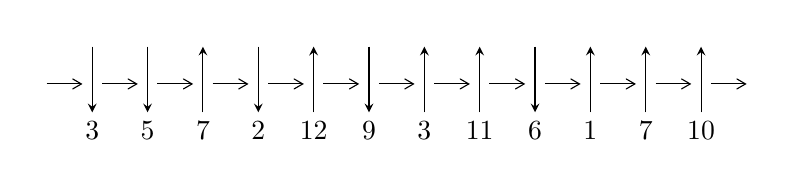
\begin{tikzpicture}[x=20pt, y=17pt]
	% nodes
	\node (C0) at (0, 0) {};
	\node (C1) at (1, 0) {};
	\node (C1U) at (1, +1) {};
	\node (C1D) at (1, -1) {3};

	\node (C2) at (2, 0) {};
	\node (C2U) at (2, +1) {};
	\node (C2D) at (2, -1) {5};

	\node (C3) at (3, 0) {};
	\node (C3U) at (3, +1) {};
	\node (C3D) at (3, -1) {7};

	\node (C4) at (4, 0) {};
	\node (C4U) at (4, +1) {};
	\node (C4D) at (4, -1) {2};

	\node (C5) at (5, 0) {};
	\node (C5U) at (5, +1) {};
	\node (C5D) at (5, -1) {12};

	\node (C6) at (6, 0) {};
	\node (C6U) at (6, +1) {};
	\node (C6D) at (6, -1) {9};

	\node (C7) at (7, 0) {};
	\node (C7U) at (7, +1) {};
	\node (C7D) at (7, -1) {3};

	\node (C8) at (8, 0) {};
	\node (C8U) at (8, +1) {};
	\node (C8D) at (8, -1) {11};

	\node (C9) at (9, 0) {};
	\node (C9U) at (9, +1) {};
	\node (C9D) at (9, -1) {6};

	\node (C10) at (10, 0) {};
	\node (C10U) at (10, +1) {};
	\node (C10D) at (10, -1) {1};

	\node (C11) at (11, 0) {};
	\node (C11U) at (11, +1) {};
	\node (C11D) at (11, -1) {7};

	\node (C12) at (12, 0) {};
	\node (C12U) at (12, +1) {};
	\node (C12D) at (12, -1) {10};
	\node (C13) at (13, 0) {};

	% arrows
	\draw[->,>={angle 60}]
	(C0) edge (C1) (C1) edge (C2) (C2) edge (C3) (C3) edge (C4) (C4) edge (C5) (C5) edge (C6) (C6) edge (C7) (C7) edge (C8) (C8) edge (C9) (C9) edge (C10) (C10) edge (C11) (C11) edge (C12) (C12) edge (C13) ;	\draw[->,>=stealth]
	(C1U) edge (C1D) (C2U) edge (C2D) (C3D) edge (C3U) (C4U) edge (C4D) (C5D) edge (C5U) (C6U) edge (C6D) (C7D) edge (C7U) (C8D) edge (C8U) (C9U) edge (C9D) (C10D) edge (C10U) (C11D) edge (C11U) (C12D) edge (C12U) ;
	\end{tikzpicture} \\
\hhline{~~} \\& 
\textbf{Solving Sequence} \\ \cline{2-2} 
 &
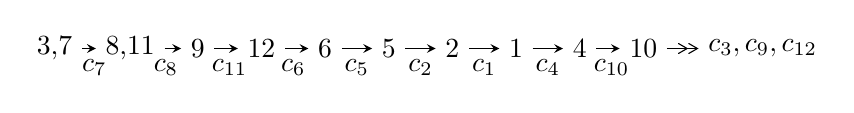
\begin{tikzpicture}[x=23pt, y=7pt]
	% node
	\node (A0) at (-1/8, 0) {3,7};
	\node (A1) at (17/16, 0) {8,11};
	\node (A2) at (17/8, 0) {9};
	\node (A3) at (25/8, 0) {12};
	\node (A4) at (33/8, 0) {6};
	\node (A5) at (41/8, 0) {5};
	\node (A6) at (49/8, 0) {2};
	\node (A7) at (57/8, 0) {1};
	\node (A8) at (65/8, 0) {4};
	\node (A9) at (73/8, 0) {10};
	\node (C1) at (1/2, -1) {$c_{7}$};
	\node (C2) at (13/8, -1) {$c_{8}$};
	\node (C3) at (21/8, -1) {$c_{11}$};
	\node (C4) at (29/8, -1) {$c_{6}$};
	\node (C5) at (37/8, -1) {$c_{5}$};
	\node (C6) at (45/8, -1) {$c_{2}$};
	\node (C7) at (53/8, -1) {$c_{1}$};
	\node (C8) at (61/8, -1) {$c_{4}$};
	\node (C9) at (69/8, -1) {$c_{10}$};
	\node (A10) at (11, 0) {$c_{3},c_{9},c_{12}$};

	% edge
	\draw[->,>=stealth]	
	(A0) edge (A1) (A1) edge (A2) (A2) edge (A3) (A3) edge (A4) (A4) edge (A5) (A5) edge (A6) (A6) edge (A7) (A7) edge (A8) (A8) edge (A9) ;
	\draw[->>,>={angle 60}]	
	(A9) edge (A10);
\end{tikzpicture} \\ 

\end{tabular} \\

\footnotetext{
The image of knot diagram is generated by the software ``\textbf{Draw programme}" developed by Andrew Bartholomew(\url{http://www.layer8.co.uk/maths/draw/index.htm\#Running-draw}), where we modified some parts for our purpose(\url{https://github.com/CATsTAILs/LinksPainter}).
}\phantom \\ \newline 
\centering \textbf{Ideals for irreducible components\footnotemark of $X_{\text{par}}$} 
 
\begin{align*}
I^u_{1}&=\langle 
5.42478\times10^{238} u^{70}-6.98254\times10^{238} u^{69}+\cdots+1.26682\times10^{239} b-3.55544\times10^{241},\\
\phantom{I^u_{1}}&\phantom{= \langle  }1.09913\times10^{240} u^{70}-2.05633\times10^{240} u^{69}+\cdots+2.15359\times10^{240} a-2.29980\times10^{243},\\
\phantom{I^u_{1}}&\phantom{= \langle  }u^{71}-2 u^{70}+\cdots-3584 u+512\rangle \\
I^u_{2}&=\langle 
b,\;9 u^4-4 u^3+3 u^2+17 a-18 u+1,\;u^5+u^4+2 u^3+u^2+u+1\rangle \\
\\
I^v_{1}&=\langle 
a,\;16726 v^8-41423 v^7+\cdots+11959 b+26601,\\
\phantom{I^v_{1}}&\phantom{= \langle  }v^9-3 v^8-2 v^7-6 v^6+25 v^5-11 v^4-9 v^3+2 v^2+3 v-1\rangle \\
\end{align*}
\raggedright * 3 irreducible components of $\dim_{\mathbb{C}}=0$, with total 85 representations.\\
\footnotetext{All coefficients of polynomials are rational numbers. But the coefficients are sometimes approximated in decimal forms when there is not enough margin.}
\newpage
\renewcommand{\arraystretch}{1}
\centering \section*{I. $I^u_{1}= \langle 5.42\times10^{238} u^{70}-6.98\times10^{238} u^{69}+\cdots+1.27\times10^{239} b-3.56\times10^{241},\;1.10\times10^{240} u^{70}-2.06\times10^{240} u^{69}+\cdots+2.15\times10^{240} a-2.30\times10^{243},\;u^{71}-2 u^{70}+\cdots-3584 u+512 \rangle$}
\flushleft \textbf{(i) Arc colorings}\\
\begin{tabular}{m{7pt} m{180pt} m{7pt} m{180pt} }
\flushright $a_{3}=$&$\begin{pmatrix}0\\u\end{pmatrix}$ \\
\flushright $a_{7}=$&$\begin{pmatrix}1\\0\end{pmatrix}$ \\
\flushright $a_{8}=$&$\begin{pmatrix}1\\- u^2\end{pmatrix}$ \\
\flushright $a_{11}=$&$\begin{pmatrix}-0.510370 u^{70}+0.954840 u^{69}+\cdots-3684.20 u+1067.89\\-0.428222 u^{70}+0.551187 u^{69}+\cdots-1698.21 u+280.659\end{pmatrix}$ \\
\flushright $a_{9}=$&$\begin{pmatrix}-0.479721 u^{70}+0.835639 u^{69}+\cdots-3127.86 u+850.474\\-0.541913 u^{70}+0.734975 u^{69}+\cdots-2349.21 u+422.606\end{pmatrix}$ \\
\flushright $a_{12}=$&$\begin{pmatrix}-0.938592 u^{70}+1.50603 u^{69}+\cdots-5382.41 u+1348.55\\-0.428222 u^{70}+0.551187 u^{69}+\cdots-1698.21 u+280.659\end{pmatrix}$ \\
\flushright $a_{6}=$&$\begin{pmatrix}0.553572 u^{70}-0.765321 u^{69}+\cdots+2500.77 u-485.024\\0.500931 u^{70}-0.690180 u^{69}+\cdots+2222.19 u-412.967\end{pmatrix}$ \\
\flushright $a_{5}=$&$\begin{pmatrix}-0.0335810 u^{70}+0.118905 u^{69}+\cdots-557.136 u+207.295\\0.242484 u^{70}-0.321369 u^{69}+\cdots+1009.04 u-176.830\end{pmatrix}$ \\
\flushright $a_{2}=$&$\begin{pmatrix}0.276065 u^{70}-0.440274 u^{69}+\cdots+1566.18 u-384.125\\0.242484 u^{70}-0.321369 u^{69}+\cdots+1009.04 u-176.830\end{pmatrix}$ \\
\flushright $a_{1}=$&$\begin{pmatrix}0.276065 u^{70}-0.440274 u^{69}+\cdots+1566.18 u-384.125\\0.192358 u^{70}-0.245562 u^{69}+\cdots+749.492 u-119.559\end{pmatrix}$ \\
\flushright $a_{4}=$&$\begin{pmatrix}u\\u\end{pmatrix}$ \\
\flushright $a_{10}=$&$\begin{pmatrix}-0.307087 u^{70}+0.617884 u^{69}+\cdots-2458.59 u+752.034\\-0.192358 u^{70}+0.245562 u^{69}+\cdots-749.492 u+119.559\end{pmatrix}$\\&\end{tabular}
\flushleft \textbf{(ii) Obstruction class $= -1$}\\~\\
\flushleft \textbf{(iii) Cusp Shapes $= 2.22925 u^{70}-3.84779 u^{69}+\cdots+14361.8 u-3919.67$}\\~\\
\newpage\renewcommand{\arraystretch}{1}
\flushleft \textbf{(iv) u-Polynomials at the component}\newline \\
\begin{tabular}{m{50pt}|m{274pt}}
Crossings & \hspace{64pt}u-Polynomials at each crossing \\
\hline $$\begin{aligned}c_{1}\end{aligned}$$&$\begin{aligned}
&u^{71}+27 u^{70}+\cdots+121 u+1
\end{aligned}$\\
\hline $$\begin{aligned}c_{2},c_{4}\end{aligned}$$&$\begin{aligned}
&u^{71}-11 u^{70}+\cdots+17 u-1
\end{aligned}$\\
\hline $$\begin{aligned}c_{3},c_{7}\end{aligned}$$&$\begin{aligned}
&u^{71}-2 u^{70}+\cdots-3584 u+512
\end{aligned}$\\
\hline $$\begin{aligned}c_{5}\end{aligned}$$&$\begin{aligned}
&17(17 u^{71}+58 u^{70}+\cdots-338322 u-76541)
\end{aligned}$\\
\hline $$\begin{aligned}c_{6},c_{9}\end{aligned}$$&$\begin{aligned}
&u^{71}-3 u^{70}+\cdots-3 u+1
\end{aligned}$\\
\hline $$\begin{aligned}c_{8}\end{aligned}$$&$\begin{aligned}
&17(17 u^{71}-28 u^{70}+\cdots-3303678 u-843836)
\end{aligned}$\\
\hline $$\begin{aligned}c_{10},c_{12}\end{aligned}$$&$\begin{aligned}
&u^{71}+7 u^{70}+\cdots+1199 u+289
\end{aligned}$\\
\hline $$\begin{aligned}c_{11}\end{aligned}$$&$\begin{aligned}
&u^{71}-2 u^{70}+\cdots-33184 u-9248
\end{aligned}$\\
\hline
\end{tabular}\\~\\
\newpage\renewcommand{\arraystretch}{1}
\flushleft \textbf{(v) Riley Polynomials at the component}\newline \\
\begin{tabular}{m{50pt}|m{274pt}}
Crossings & \hspace{64pt}Riley Polynomials at each crossing \\
\hline $$\begin{aligned}c_{1}\end{aligned}$$&$\begin{aligned}
&y^{71}+45 y^{70}+\cdots+15729 y-1
\end{aligned}$\\
\hline $$\begin{aligned}c_{2},c_{4}\end{aligned}$$&$\begin{aligned}
&y^{71}-27 y^{70}+\cdots+121 y-1
\end{aligned}$\\
\hline $$\begin{aligned}c_{3},c_{7}\end{aligned}$$&$\begin{aligned}
&y^{71}-54 y^{70}+\cdots+10485760 y-262144
\end{aligned}$\\
\hline $$\begin{aligned}c_{5}\end{aligned}$$&$\begin{aligned}
&289(289 y^{71}-11218 y^{70}+\cdots+5.96694\times10^{10} y-5.85852\times10^{9})
\end{aligned}$\\
\hline $$\begin{aligned}c_{6},c_{9}\end{aligned}$$&$\begin{aligned}
&y^{71}+49 y^{70}+\cdots+41 y-1
\end{aligned}$\\
\hline $$\begin{aligned}c_{8}\end{aligned}$$&$\begin{aligned}
&289\\
&\cdot(289 y^{71}-16424 y^{70}+\cdots+1192944884236 y-712059194896)
\end{aligned}$\\
\hline $$\begin{aligned}c_{10},c_{12}\end{aligned}$$&$\begin{aligned}
&y^{71}-63 y^{70}+\cdots+1811567 y-83521
\end{aligned}$\\
\hline $$\begin{aligned}c_{11}\end{aligned}$$&$\begin{aligned}
&y^{71}-30 y^{70}+\cdots+374507008 y-85525504
\end{aligned}$\\
\hline
\end{tabular}\\~\\
\newpage\flushleft \textbf{(vi) Complex Volumes and Cusp Shapes}
$$\begin{array}{c|c|c}  
\text{Solutions to }I^u_{1}& \I (\text{vol} + \sqrt{-1}CS) & \text{Cusp shape}\\
 \hline 
\begin{aligned}
u &= \phantom{-}0.076693 + 0.947370 I \\
a &= -0.691781 - 0.148799 I \\
b &= -1.37182 + 0.60834 I\end{aligned}
 & \phantom{-}1.59411 - 4.42837 I & \phantom{-0.000000 } 0 \\ \hline\begin{aligned}
u &= \phantom{-}0.076693 - 0.947370 I \\
a &= -0.691781 + 0.148799 I \\
b &= -1.37182 - 0.60834 I\end{aligned}
 & \phantom{-}1.59411 + 4.42837 I & \phantom{-0.000000 } 0 \\ \hline\begin{aligned}
u &= -0.220480 + 0.816559 I \\
a &= \phantom{-}0.463726 + 0.218399 I \\
b &= \phantom{-}0.558026 + 0.462831 I\end{aligned}
 & -1.56511 + 1.33089 I & -4.35474 - 3.35992 I \\ \hline\begin{aligned}
u &= -0.220480 - 0.816559 I \\
a &= \phantom{-}0.463726 - 0.218399 I \\
b &= \phantom{-}0.558026 - 0.462831 I\end{aligned}
 & -1.56511 - 1.33089 I & -4.35474 + 3.35992 I \\ \hline\begin{aligned}
u &= \phantom{-}0.145194 + 0.788536 I \\
a &= -0.516702 + 1.147430 I \\
b &= -0.761187 - 0.160663 I\end{aligned}
 & \phantom{-}1.32199 + 0.86803 I & \phantom{-}2.81463 + 0.68879 I \\ \hline\begin{aligned}
u &= \phantom{-}0.145194 - 0.788536 I \\
a &= -0.516702 - 1.147430 I \\
b &= -0.761187 + 0.160663 I\end{aligned}
 & \phantom{-}1.32199 - 0.86803 I & \phantom{-}2.81463 - 0.68879 I \\ \hline\begin{aligned}
u &= -0.487435 + 1.128170 I \\
a &= \phantom{-}0.0239672 - 0.0816915 I \\
b &= \phantom{-}0.080432 + 0.375354 I\end{aligned}
 & -4.36546 - 4.32846 I & \phantom{-0.000000 } 0 \\ \hline\begin{aligned}
u &= -0.487435 - 1.128170 I \\
a &= \phantom{-}0.0239672 + 0.0816915 I \\
b &= \phantom{-}0.080432 - 0.375354 I\end{aligned}
 & -4.36546 + 4.32846 I & \phantom{-0.000000 } 0 \\ \hline\begin{aligned}
u &= \phantom{-}0.439418 + 0.621478 I \\
a &= \phantom{-}0.206543 + 0.342654 I \\
b &= -0.047968 - 0.545007 I\end{aligned}
 & \phantom{-}0.12984 + 1.53500 I & \phantom{-}0.43134 - 4.26020 I \\ \hline\begin{aligned}
u &= \phantom{-}0.439418 - 0.621478 I \\
a &= \phantom{-}0.206543 - 0.342654 I \\
b &= -0.047968 + 0.545007 I\end{aligned}
 & \phantom{-}0.12984 - 1.53500 I & \phantom{-}0.43134 + 4.26020 I\\
 \hline 
 \end{array}$$\newpage$$\begin{array}{c|c|c}  
\text{Solutions to }I^u_{1}& \I (\text{vol} + \sqrt{-1}CS) & \text{Cusp shape}\\
 \hline 
\begin{aligned}
u &= \phantom{-}0.182323 + 0.721295 I \\
a &= \phantom{-}0.56676 - 2.11337 I \\
b &= \phantom{-}0.74195 - 1.33427 I\end{aligned}
 & \phantom{-}4.92838 + 1.62527 I & \phantom{-}9.65649 - 3.98384 I \\ \hline\begin{aligned}
u &= \phantom{-}0.182323 - 0.721295 I \\
a &= \phantom{-}0.56676 + 2.11337 I \\
b &= \phantom{-}0.74195 + 1.33427 I\end{aligned}
 & \phantom{-}4.92838 - 1.62527 I & \phantom{-}9.65649 + 3.98384 I \\ \hline\begin{aligned}
u &= \phantom{-}0.738712 + 0.025801 I \\
a &= -2.84205 + 2.51257 I \\
b &= \phantom{-}0.986916 - 0.482298 I\end{aligned}
 & \phantom{-}0.03593 - 2.58057 I & \phantom{-}5.84465 + 3.57644 I \\ \hline\begin{aligned}
u &= \phantom{-}0.738712 - 0.025801 I \\
a &= -2.84205 - 2.51257 I \\
b &= \phantom{-}0.986916 + 0.482298 I\end{aligned}
 & \phantom{-}0.03593 + 2.58057 I & \phantom{-}5.84465 - 3.57644 I \\ \hline\begin{aligned}
u &= -0.642897 + 0.339317 I \\
a &= \phantom{-}1.63273 - 0.52748 I \\
b &= -0.210241 + 0.516302 I\end{aligned}
 & -2.40004 + 0.50009 I & -3.16242 + 1.54853 I \\ \hline\begin{aligned}
u &= -0.642897 - 0.339317 I \\
a &= \phantom{-}1.63273 + 0.52748 I \\
b &= -0.210241 - 0.516302 I\end{aligned}
 & -2.40004 - 0.50009 I & -3.16242 - 1.54853 I \\ \hline\begin{aligned}
u &= -1.323750 + 0.085283 I \\
a &= -1.90895 + 0.72230 I \\
b &= \phantom{-}0.663197 - 0.063213 I\end{aligned}
 & \phantom{-}5.87495 - 2.45786 I & \phantom{-0.000000 } 0 \\ \hline\begin{aligned}
u &= -1.323750 - 0.085283 I \\
a &= -1.90895 - 0.72230 I \\
b &= \phantom{-}0.663197 + 0.063213 I\end{aligned}
 & \phantom{-}5.87495 + 2.45786 I & \phantom{-0.000000 } 0 \\ \hline\begin{aligned}
u &= -0.004372 + 0.661805 I \\
a &= \phantom{-}1.40629 - 2.21793 I \\
b &= -0.395556 - 0.414217 I\end{aligned}
 & \phantom{-}0.982639 - 0.712583 I & \phantom{-}1.26468 - 3.38200 I \\ \hline\begin{aligned}
u &= -0.004372 - 0.661805 I \\
a &= \phantom{-}1.40629 + 2.21793 I \\
b &= -0.395556 + 0.414217 I\end{aligned}
 & \phantom{-}0.982639 + 0.712583 I & \phantom{-}1.26468 + 3.38200 I\\
 \hline 
 \end{array}$$\newpage$$\begin{array}{c|c|c}  
\text{Solutions to }I^u_{1}& \I (\text{vol} + \sqrt{-1}CS) & \text{Cusp shape}\\
 \hline 
\begin{aligned}
u &= \phantom{-}1.354200 + 0.058471 I \\
a &= \phantom{-}1.169270 + 0.041829 I \\
b &= -1.151030 - 0.496491 I\end{aligned}
 & \phantom{-}3.26913 + 0.37177 I & \phantom{-0.000000 } 0 \\ \hline\begin{aligned}
u &= \phantom{-}1.354200 - 0.058471 I \\
a &= \phantom{-}1.169270 - 0.041829 I \\
b &= -1.151030 + 0.496491 I\end{aligned}
 & \phantom{-}3.26913 - 0.37177 I & \phantom{-0.000000 } 0 \\ \hline\begin{aligned}
u &= \phantom{-}0.641537 + 0.013263 I \\
a &= -0.215156 + 0.261484 I \\
b &= -0.477396 - 1.105930 I\end{aligned}
 & -0.01259 + 2.24943 I & \phantom{-}5.94216 - 1.24752 I \\ \hline\begin{aligned}
u &= \phantom{-}0.641537 - 0.013263 I \\
a &= -0.215156 - 0.261484 I \\
b &= -0.477396 + 1.105930 I\end{aligned}
 & -0.01259 - 2.24943 I & \phantom{-}5.94216 + 1.24752 I \\ \hline\begin{aligned}
u &= -0.637235 + 0.065847 I \\
a &= \phantom{-}0.146928 + 0.026378 I \\
b &= -0.083520 + 1.139150 I\end{aligned}
 & -2.82440 - 2.46359 I & \phantom{-}4.30273 + 6.24454 I \\ \hline\begin{aligned}
u &= -0.637235 - 0.065847 I \\
a &= \phantom{-}0.146928 - 0.026378 I \\
b &= -0.083520 - 1.139150 I\end{aligned}
 & -2.82440 + 2.46359 I & \phantom{-}4.30273 - 6.24454 I \\ \hline\begin{aligned}
u &= \phantom{-}1.334450 + 0.351523 I \\
a &= -1.13740 + 0.91626 I \\
b &= \phantom{-}0.663249 + 0.125810 I\end{aligned}
 & \phantom{-}5.32732 + 3.31503 I & \phantom{-0.000000 } 0 \\ \hline\begin{aligned}
u &= \phantom{-}1.334450 - 0.351523 I \\
a &= -1.13740 - 0.91626 I \\
b &= \phantom{-}0.663249 - 0.125810 I\end{aligned}
 & \phantom{-}5.32732 - 3.31503 I & \phantom{-0.000000 } 0 \\ \hline\begin{aligned}
u &= \phantom{-}1.392010 + 0.087028 I \\
a &= \phantom{-}1.235080 - 0.640698 I \\
b &= -1.231910 + 0.578737 I\end{aligned}
 & \phantom{-}5.60335 - 6.26016 I & \phantom{-0.000000 } 0 \\ \hline\begin{aligned}
u &= \phantom{-}1.392010 - 0.087028 I \\
a &= \phantom{-}1.235080 + 0.640698 I \\
b &= -1.231910 - 0.578737 I\end{aligned}
 & \phantom{-}5.60335 + 6.26016 I & \phantom{-0.000000 } 0\\
 \hline 
 \end{array}$$\newpage$$\begin{array}{c|c|c}  
\text{Solutions to }I^u_{1}& \I (\text{vol} + \sqrt{-1}CS) & \text{Cusp shape}\\
 \hline 
\begin{aligned}
u &= -0.426783 + 0.400297 I \\
a &= \phantom{-}4.22729 + 5.26355 I \\
b &= -0.290627 + 0.848259 I\end{aligned}
 & \phantom{-}2.71880 + 0.77171 I & -0.03938 + 7.34337 I \\ \hline\begin{aligned}
u &= -0.426783 - 0.400297 I \\
a &= \phantom{-}4.22729 - 5.26355 I \\
b &= -0.290627 - 0.848259 I\end{aligned}
 & \phantom{-}2.71880 - 0.77171 I & -0.03938 - 7.34337 I \\ \hline\begin{aligned}
u &= \phantom{-}0.557977 + 0.073436 I \\
a &= -0.051806 + 0.142442 I \\
b &= \phantom{-}0.646310 + 1.044790 I\end{aligned}
 & \phantom{-}2.38069 + 7.27157 I & \phantom{-}12.6640 - 9.5899 I \\ \hline\begin{aligned}
u &= \phantom{-}0.557977 - 0.073436 I \\
a &= -0.051806 - 0.142442 I \\
b &= \phantom{-}0.646310 - 1.044790 I\end{aligned}
 & \phantom{-}2.38069 - 7.27157 I & \phantom{-}12.6640 + 9.5899 I \\ \hline\begin{aligned}
u &= -1.43718 + 0.15590 I \\
a &= -0.944374 - 0.509182 I \\
b &= \phantom{-}0.480613 - 0.961739 I\end{aligned}
 & \phantom{-}6.20644 - 1.78085 I & \phantom{-0.000000 } 0 \\ \hline\begin{aligned}
u &= -1.43718 - 0.15590 I \\
a &= -0.944374 + 0.509182 I \\
b &= \phantom{-}0.480613 + 0.961739 I\end{aligned}
 & \phantom{-}6.20644 + 1.78085 I & \phantom{-0.000000 } 0 \\ \hline\begin{aligned}
u &= -1.37199 + 0.46590 I \\
a &= \phantom{-}1.173090 + 0.216321 I \\
b &= -1.073480 + 0.872449 I\end{aligned}
 & \phantom{-}2.23860 - 6.33244 I & \phantom{-0.000000 } 0 \\ \hline\begin{aligned}
u &= -1.37199 - 0.46590 I \\
a &= \phantom{-}1.173090 - 0.216321 I \\
b &= -1.073480 - 0.872449 I\end{aligned}
 & \phantom{-}2.23860 + 6.33244 I & \phantom{-0.000000 } 0 \\ \hline\begin{aligned}
u &= \phantom{-}0.16002 + 1.45030 I \\
a &= -0.0471063 - 0.1086940 I \\
b &= \phantom{-}1.33837 - 0.76483 I\end{aligned}
 & \phantom{-}7.57456 - 9.33161 I & \phantom{-0.000000 } 0 \\ \hline\begin{aligned}
u &= \phantom{-}0.16002 - 1.45030 I \\
a &= -0.0471063 + 0.1086940 I \\
b &= \phantom{-}1.33837 + 0.76483 I\end{aligned}
 & \phantom{-}7.57456 + 9.33161 I & \phantom{-0.000000 } 0\\
 \hline 
 \end{array}$$\newpage$$\begin{array}{c|c|c}  
\text{Solutions to }I^u_{1}& \I (\text{vol} + \sqrt{-1}CS) & \text{Cusp shape}\\
 \hline 
\begin{aligned}
u &= \phantom{-}1.44190 + 0.27798 I \\
a &= -0.928627 - 0.073907 I \\
b &= \phantom{-}0.768169 - 0.880679 I\end{aligned}
 & \phantom{-}5.97359 + 4.40312 I & \phantom{-0.000000 } 0 \\ \hline\begin{aligned}
u &= \phantom{-}1.44190 - 0.27798 I \\
a &= -0.928627 + 0.073907 I \\
b &= \phantom{-}0.768169 + 0.880679 I\end{aligned}
 & \phantom{-}5.97359 - 4.40312 I & \phantom{-0.000000 } 0 \\ \hline\begin{aligned}
u &= -1.47168 + 0.09988 I \\
a &= -1.48841 + 0.33110 I \\
b &= \phantom{-}2.07259 - 0.81942 I\end{aligned}
 & \phantom{-}7.18645 - 3.56652 I & \phantom{-0.000000 } 0 \\ \hline\begin{aligned}
u &= -1.47168 - 0.09988 I \\
a &= -1.48841 - 0.33110 I \\
b &= \phantom{-}2.07259 + 0.81942 I\end{aligned}
 & \phantom{-}7.18645 + 3.56652 I & \phantom{-0.000000 } 0 \\ \hline\begin{aligned}
u &= -0.420831 + 0.275485 I \\
a &= -0.74354 - 2.33627 I \\
b &= \phantom{-}1.032730 - 0.604659 I\end{aligned}
 & \phantom{-}4.35121 + 1.59493 I & \phantom{-}10.43394 - 0.97479 I \\ \hline\begin{aligned}
u &= -0.420831 - 0.275485 I \\
a &= -0.74354 + 2.33627 I \\
b &= \phantom{-}1.032730 + 0.604659 I\end{aligned}
 & \phantom{-}4.35121 - 1.59493 I & \phantom{-}10.43394 + 0.97479 I \\ \hline\begin{aligned}
u &= \phantom{-}0.30543 + 1.48272 I \\
a &= -0.0549019 + 0.1030280 I \\
b &= \phantom{-}1.245940 + 0.346093 I\end{aligned}
 & \phantom{-}7.30098 + 3.05381 I & \phantom{-0.000000 } 0 \\ \hline\begin{aligned}
u &= \phantom{-}0.30543 - 1.48272 I \\
a &= -0.0549019 - 0.1030280 I \\
b &= \phantom{-}1.245940 - 0.346093 I\end{aligned}
 & \phantom{-}7.30098 - 3.05381 I & \phantom{-0.000000 } 0 \\ \hline\begin{aligned}
u &= -1.51898\phantom{ +0.000000I} \\
a &= -0.897992\phantom{ +0.000000I} \\
b &= \phantom{-}0.945902\phantom{ +0.000000I}\end{aligned}
 & \phantom{-}0.852763\phantom{ +0.000000I} & \phantom{-0.000000 } 0 \\ \hline\begin{aligned}
u &= \phantom{-}1.45011 + 0.48802 I \\
a &= -1.53939 + 0.17087 I \\
b &= \phantom{-}1.89726 + 1.26956 I\end{aligned}
 & \phantom{-}6.09358 + 9.90312 I & \phantom{-0.000000 } 0\\
 \hline 
 \end{array}$$\newpage$$\begin{array}{c|c|c}  
\text{Solutions to }I^u_{1}& \I (\text{vol} + \sqrt{-1}CS) & \text{Cusp shape}\\
 \hline 
\begin{aligned}
u &= \phantom{-}1.45011 - 0.48802 I \\
a &= -1.53939 - 0.17087 I \\
b &= \phantom{-}1.89726 - 1.26956 I\end{aligned}
 & \phantom{-}6.09358 - 9.90312 I & \phantom{-0.000000 } 0 \\ \hline\begin{aligned}
u &= \phantom{-}1.55039 + 0.12499 I \\
a &= \phantom{-}1.120780 + 0.568665 I \\
b &= -1.42403 - 2.23704 I\end{aligned}
 & \phantom{-}11.13970 + 0.68264 I & \phantom{-0.000000 } 0 \\ \hline\begin{aligned}
u &= \phantom{-}1.55039 - 0.12499 I \\
a &= \phantom{-}1.120780 - 0.568665 I \\
b &= -1.42403 + 2.23704 I\end{aligned}
 & \phantom{-}11.13970 - 0.68264 I & \phantom{-0.000000 } 0 \\ \hline\begin{aligned}
u &= -0.18896 + 1.55398 I \\
a &= \phantom{-}0.0798087 + 0.0002794 I \\
b &= -1.030510 - 0.264735 I\end{aligned}
 & \phantom{-}2.79580 + 3.31170 I & \phantom{-0.000000 } 0 \\ \hline\begin{aligned}
u &= -0.18896 - 1.55398 I \\
a &= \phantom{-}0.0798087 - 0.0002794 I \\
b &= -1.030510 + 0.264735 I\end{aligned}
 & \phantom{-}2.79580 - 3.31170 I & \phantom{-0.000000 } 0 \\ \hline\begin{aligned}
u &= -1.53761 + 0.31028 I \\
a &= \phantom{-}0.757396 + 0.910802 I \\
b &= -1.86995 - 1.88969 I\end{aligned}
 & \phantom{-}10.80380 - 5.89219 I & \phantom{-0.000000 } 0 \\ \hline\begin{aligned}
u &= -1.53761 - 0.31028 I \\
a &= \phantom{-}0.757396 - 0.910802 I \\
b &= -1.86995 + 1.88969 I\end{aligned}
 & \phantom{-}10.80380 + 5.89219 I & \phantom{-0.000000 } 0 \\ \hline\begin{aligned}
u &= \phantom{-}1.50255 + 0.73985 I \\
a &= \phantom{-}1.331380 - 0.402936 I \\
b &= -1.43302 - 1.19081 I\end{aligned}
 & \phantom{-}11.7776 + 17.0387 I & \phantom{-0.000000 } 0 \\ \hline\begin{aligned}
u &= \phantom{-}1.50255 - 0.73985 I \\
a &= \phantom{-}1.331380 + 0.402936 I \\
b &= -1.43302 + 1.19081 I\end{aligned}
 & \phantom{-}11.7776 - 17.0387 I & \phantom{-0.000000 } 0 \\ \hline\begin{aligned}
u &= \phantom{-}0.310196\phantom{ +0.000000I} \\
a &= -11.7418\phantom{ +0.000000I} \\
b &= \phantom{-}0.360541\phantom{ +0.000000I}\end{aligned}
 & -0.278739\phantom{ +0.000000I} & \phantom{-}56.4200\phantom{ +0.000000I}\\
 \hline 
 \end{array}$$\newpage$$\begin{array}{c|c|c}  
\text{Solutions to }I^u_{1}& \I (\text{vol} + \sqrt{-1}CS) & \text{Cusp shape}\\
 \hline 
\begin{aligned}
u &= \phantom{-}0.297760\phantom{ +0.000000I} \\
a &= \phantom{-}2.27908\phantom{ +0.000000I} \\
b &= -0.569710\phantom{ +0.000000I}\end{aligned}
 & \phantom{-}1.11352\phantom{ +0.000000I} & \phantom{-}9.05470\phantom{ +0.000000I} \\ \hline\begin{aligned}
u &= -1.53644 + 0.75409 I \\
a &= -1.045060 - 0.283594 I \\
b &= \phantom{-}1.17961 - 0.86678 I\end{aligned}
 & \phantom{-}7.10450 - 11.36750 I & \phantom{-0.000000 } 0 \\ \hline\begin{aligned}
u &= -1.53644 - 0.75409 I \\
a &= -1.045060 + 0.283594 I \\
b &= \phantom{-}1.17961 + 0.86678 I\end{aligned}
 & \phantom{-}7.10450 + 11.36750 I & \phantom{-0.000000 } 0 \\ \hline\begin{aligned}
u &= -1.66767 + 0.47111 I \\
a &= \phantom{-}1.258780 + 0.087385 I \\
b &= -1.54465 + 0.98213 I\end{aligned}
 & \phantom{-}13.8741 - 10.1106 I & \phantom{-0.000000 } 0 \\ \hline\begin{aligned}
u &= -1.66767 - 0.47111 I \\
a &= \phantom{-}1.258780 - 0.087385 I \\
b &= -1.54465 - 0.98213 I\end{aligned}
 & \phantom{-}13.8741 + 10.1106 I & \phantom{-0.000000 } 0 \\ \hline\begin{aligned}
u &= \phantom{-}1.52848 + 0.82309 I \\
a &= \phantom{-}0.679890 - 0.444350 I \\
b &= -1.200100 - 0.331040 I\end{aligned}
 & \phantom{-}11.07870 + 5.15354 I & \phantom{-0.000000 } 0 \\ \hline\begin{aligned}
u &= \phantom{-}1.52848 - 0.82309 I \\
a &= \phantom{-}0.679890 + 0.444350 I \\
b &= -1.200100 + 0.331040 I\end{aligned}
 & \phantom{-}11.07870 - 5.15354 I & \phantom{-0.000000 } 0 \\ \hline\begin{aligned}
u &= -1.68752 + 0.56968 I \\
a &= \phantom{-}0.767625 + 0.443423 I \\
b &= -1.41908 + 0.00115 I\end{aligned}
 & \phantom{-}13.45460 + 1.92659 I & \phantom{-0.000000 } 0 \\ \hline\begin{aligned}
u &= -1.68752 - 0.56968 I \\
a &= \phantom{-}0.767625 - 0.443423 I \\
b &= -1.41908 - 0.00115 I\end{aligned}
 & \phantom{-}13.45460 - 1.92659 I & \phantom{-0.000000 } 0 \\ \hline\begin{aligned}
u &= \phantom{-}1.71694 + 0.49452 I \\
a &= -0.955855 + 0.132868 I \\
b &= \phantom{-}1.292340 + 0.569757 I\end{aligned}
 & \phantom{-}9.22845 + 4.28954 I & \phantom{-0.000000 } 0\\
 \hline 
 \end{array}$$\newpage$$\begin{array}{c|c|c}  
\text{Solutions to }I^u_{1}& \I (\text{vol} + \sqrt{-1}CS) & \text{Cusp shape}\\
 \hline 
\begin{aligned}
u &= \phantom{-}1.71694 - 0.49452 I \\
a &= -0.955855 - 0.132868 I \\
b &= \phantom{-}1.292340 - 0.569757 I\end{aligned}
 & \phantom{-}9.22845 - 4.28954 I & \phantom{-0.000000 } 0\\
 \hline 
 \end{array}$$\newpage\newpage\renewcommand{\arraystretch}{1}
\centering \section*{II. $I^u_{2}= \langle b,\;9 u^4-4 u^3+3 u^2+17 a-18 u+1,\;u^5+u^4+2 u^3+u^2+u+1 \rangle$}
\flushleft \textbf{(i) Arc colorings}\\
\begin{tabular}{m{7pt} m{180pt} m{7pt} m{180pt} }
\flushright $a_{3}=$&$\begin{pmatrix}0\\u\end{pmatrix}$ \\
\flushright $a_{7}=$&$\begin{pmatrix}1\\0\end{pmatrix}$ \\
\flushright $a_{8}=$&$\begin{pmatrix}1\\- u^2\end{pmatrix}$ \\
\flushright $a_{11}=$&$\begin{pmatrix}-0.529412 u^{4}+0.235294 u^{3}+\cdots+1.05882 u-0.0588235\\0\end{pmatrix}$ \\
\flushright $a_{9}=$&$\begin{pmatrix}-0.131488 u^{4}+0.463668 u^{3}+\cdots+0.910035 u+0.854671\\- u^2\end{pmatrix}$ \\
\flushright $a_{12}=$&$\begin{pmatrix}-0.529412 u^{4}+0.235294 u^{3}+\cdots+1.05882 u-0.0588235\\0\end{pmatrix}$ \\
\flushright $a_{6}=$&$\begin{pmatrix}-0.0622837 u^{4}-0.148789 u^{3}+\cdots-0.463668 u+0.404844\\- u^4\end{pmatrix}$ \\
\flushright $a_{5}=$&$\begin{pmatrix}u^2+1\\- u^4\end{pmatrix}$ \\
\flushright $a_{2}=$&$\begin{pmatrix}- u^4- u^2-1\\- u^4\end{pmatrix}$ \\
\flushright $a_{1}=$&$\begin{pmatrix}- u^4- u^2-1\\- u^4+u^3+u^2+1\end{pmatrix}$ \\
\flushright $a_{4}=$&$\begin{pmatrix}u\\u\end{pmatrix}$ \\
\flushright $a_{10}=$&$\begin{pmatrix}0.470588 u^{4}+0.235294 u^{3}+\cdots+1.05882 u+0.941176\\u^4- u^3- u^2-1\end{pmatrix}$\\&\end{tabular}
\flushleft \textbf{(ii) Obstruction class $= 1$}\\~\\
\flushleft \textbf{(iii) Cusp Shapes $= \frac{1429}{289} u^4+\frac{1471}{289} u^3-\frac{1184}{289} u^2+\frac{780}{289} u+\frac{2127}{289}$}\\~\\
\newpage\renewcommand{\arraystretch}{1}
\flushleft \textbf{(iv) u-Polynomials at the component}\newline \\
\begin{tabular}{m{50pt}|m{274pt}}
Crossings & \hspace{64pt}u-Polynomials at each crossing \\
\hline $$\begin{aligned}c_{1}\end{aligned}$$&$\begin{aligned}
&u^5-5 u^4+8 u^3-3 u^2- u-1
\end{aligned}$\\
\hline $$\begin{aligned}c_{2}\end{aligned}$$&$\begin{aligned}
&u^5+u^4-2 u^3- u^2+u-1
\end{aligned}$\\
\hline $$\begin{aligned}c_{3}\end{aligned}$$&$\begin{aligned}
&u^5- u^4+2 u^3- u^2+u-1
\end{aligned}$\\
\hline $$\begin{aligned}c_{4}\end{aligned}$$&$\begin{aligned}
&u^5- u^4-2 u^3+u^2+u+1
\end{aligned}$\\
\hline $$\begin{aligned}c_{5}\end{aligned}$$&$\begin{aligned}
&17(17 u^5-32 u^4+18 u^3+u^2-4 u+1)
\end{aligned}$\\
\hline $$\begin{aligned}c_{6}\end{aligned}$$&$\begin{aligned}
&u^5-3 u^4+4 u^3- u^2- u+1
\end{aligned}$\\
\hline $$\begin{aligned}c_{7}\end{aligned}$$&$\begin{aligned}
&u^5+u^4+2 u^3+u^2+u+1
\end{aligned}$\\
\hline $$\begin{aligned}c_{8}\end{aligned}$$&$\begin{aligned}
&17(17 u^5+42 u^4+43 u^3+22 u^2+6 u+1)
\end{aligned}$\\
\hline $$\begin{aligned}c_{9}\end{aligned}$$&$\begin{aligned}
&u^5+3 u^4+4 u^3+u^2- u-1
\end{aligned}$\\
\hline $$\begin{aligned}c_{10}\end{aligned}$$&$\begin{aligned}
&(u+1)^5
\end{aligned}$\\
\hline $$\begin{aligned}c_{11}\end{aligned}$$&$\begin{aligned}
&u^5
\end{aligned}$\\
\hline $$\begin{aligned}c_{12}\end{aligned}$$&$\begin{aligned}
&(u-1)^5
\end{aligned}$\\
\hline
\end{tabular}\\~\\
\newpage\renewcommand{\arraystretch}{1}
\flushleft \textbf{(v) Riley Polynomials at the component}\newline \\
\begin{tabular}{m{50pt}|m{274pt}}
Crossings & \hspace{64pt}Riley Polynomials at each crossing \\
\hline $$\begin{aligned}c_{1}\end{aligned}$$&$\begin{aligned}
&y^5-9 y^4+32 y^3-35 y^2-5 y-1
\end{aligned}$\\
\hline $$\begin{aligned}c_{2},c_{4}\end{aligned}$$&$\begin{aligned}
&y^5-5 y^4+8 y^3-3 y^2- y-1
\end{aligned}$\\
\hline $$\begin{aligned}c_{3},c_{7}\end{aligned}$$&$\begin{aligned}
&y^5+3 y^4+4 y^3+y^2- y-1
\end{aligned}$\\
\hline $$\begin{aligned}c_{5}\end{aligned}$$&$\begin{aligned}
&289(289 y^5-412 y^4+252 y^3-81 y^2+14 y-1)
\end{aligned}$\\
\hline $$\begin{aligned}c_{6},c_{9}\end{aligned}$$&$\begin{aligned}
&y^5- y^4+8 y^3-3 y^2+3 y-1
\end{aligned}$\\
\hline $$\begin{aligned}c_{8}\end{aligned}$$&$\begin{aligned}
&289(289 y^5-302 y^4+205 y^3-52 y^2-8 y-1)
\end{aligned}$\\
\hline $$\begin{aligned}c_{10},c_{12}\end{aligned}$$&$\begin{aligned}
&(y-1)^5
\end{aligned}$\\
\hline $$\begin{aligned}c_{11}\end{aligned}$$&$\begin{aligned}
&y^5
\end{aligned}$\\
\hline
\end{tabular}\\~\\
\newpage\flushleft \textbf{(vi) Complex Volumes and Cusp Shapes}
$$\begin{array}{c|c|c}  
\text{Solutions to }I^u_{2}& \I (\text{vol} + \sqrt{-1}CS) & \text{Cusp shape}\\
 \hline 
\begin{aligned}
u &= \phantom{-}0.339110 + 0.822375 I \\
a &= \phantom{-}0.244471 + 1.039700 I \\
b &= \phantom{-0.000000 } 0\end{aligned}
 & \phantom{-}1.31583 + 1.53058 I & \phantom{-}7.29086 - 4.54835 I \\ \hline\begin{aligned}
u &= \phantom{-}0.339110 - 0.822375 I \\
a &= \phantom{-}0.244471 - 1.039700 I \\
b &= \phantom{-0.000000 } 0\end{aligned}
 & \phantom{-}1.31583 - 1.53058 I & \phantom{-}7.29086 + 4.54835 I \\ \hline\begin{aligned}
u &= -0.766826\phantom{ +0.000000I} \\
a &= -1.26368\phantom{ +0.000000I} \\
b &= \phantom{-0.000000 } 0\end{aligned}
 & -0.756147\phantom{ +0.000000I} & \phantom{-}2.29580\phantom{ +0.000000I} \\ \hline\begin{aligned}
u &= -0.455697 + 1.200150 I \\
a &= -0.053809 - 0.194708 I \\
b &= \phantom{-0.000000 } 0\end{aligned}
 & -4.22763 - 4.40083 I & \phantom{-}22.3190 + 16.0614 I \\ \hline\begin{aligned}
u &= -0.455697 - 1.200150 I \\
a &= -0.053809 + 0.194708 I \\
b &= \phantom{-0.000000 } 0\end{aligned}
 & -4.22763 + 4.40083 I & \phantom{-}22.3190 - 16.0614 I\\
 \hline 
 \end{array}$$\newpage\newpage\renewcommand{\arraystretch}{1}
\centering \section*{III. $I^v_{1}= \langle a,\;16726 v^8-41423 v^7+\cdots+11959 b+26601,\;v^9-3 v^8+\cdots+3 v-1 \rangle$}
\flushleft \textbf{(i) Arc colorings}\\
\begin{tabular}{m{7pt} m{180pt} m{7pt} m{180pt} }
\flushright $a_{3}=$&$\begin{pmatrix}v\\0\end{pmatrix}$ \\
\flushright $a_{7}=$&$\begin{pmatrix}1\\0\end{pmatrix}$ \\
\flushright $a_{8}=$&$\begin{pmatrix}1\\0\end{pmatrix}$ \\
\flushright $a_{11}=$&$\begin{pmatrix}0\\-1.39861 v^{8}+3.46375 v^{7}+\cdots+3.94598 v-2.22435\end{pmatrix}$ \\
\flushright $a_{9}=$&$\begin{pmatrix}1\\1.45213 v^{8}-3.82515 v^{7}+\cdots-3.73944 v+4.14098\end{pmatrix}$ \\
\flushright $a_{12}=$&$\begin{pmatrix}-1.39861 v^{8}+3.46375 v^{7}+\cdots+3.94598 v-2.22435\\-1.39861 v^{8}+3.46375 v^{7}+\cdots+3.94598 v-2.22435\end{pmatrix}$ \\
\flushright $a_{6}=$&$\begin{pmatrix}-1.45213 v^{8}+3.82515 v^{7}+\cdots+3.73944 v-3.14098\\-1.21114 v^{8}+2.94147 v^{7}+\cdots+5.63826 v-2.00702\end{pmatrix}$ \\
\flushright $a_{5}=$&$\begin{pmatrix}0.759010 v^{8}-2.11631 v^{7}+\cdots+0.101179 v+1.86604\\v^8-3 v^7-2 v^6-6 v^5+25 v^4-11 v^3-9 v^2+2 v+3\end{pmatrix}$ \\
\flushright $a_{2}=$&$\begin{pmatrix}-0.759010 v^{8}+2.11631 v^{7}+\cdots+0.898821 v-1.86604\\- v^8+3 v^7+2 v^6+6 v^5-25 v^4+11 v^3+9 v^2-2 v-3\end{pmatrix}$ \\
\flushright $a_{1}=$&$\begin{pmatrix}-0.759010 v^{8}+2.11631 v^{7}+\cdots-0.101179 v-1.86604\\- v^8+3 v^7+2 v^6+6 v^5-25 v^4+11 v^3+9 v^2-2 v-3\end{pmatrix}$ \\
\flushright $a_{4}=$&$\begin{pmatrix}v\\0\end{pmatrix}$ \\
\flushright $a_{10}=$&$\begin{pmatrix}-0.240990 v^{8}+0.883686 v^{7}+\cdots-1.89882 v-1.13396\\- v^8+3 v^7+2 v^6+6 v^5-25 v^4+11 v^3+9 v^2-2 v-3\end{pmatrix}$\\&\end{tabular}
\flushleft \textbf{(ii) Obstruction class $= 1$}\\~\\
\flushleft \textbf{(iii) Cusp Shapes $= \frac{38011}{11959} v^8-\frac{103132}{11959} v^7-\frac{110061}{11959} v^6-\frac{250712}{11959} v^5+\frac{892353}{11959} v^4-\frac{104528}{11959} v^3-\frac{444297}{11959} v^2-\frac{43711}{11959} v+\frac{44549}{11959}$}\\~\\
\newpage\renewcommand{\arraystretch}{1}
\flushleft \textbf{(iv) u-Polynomials at the component}\newline \\
\begin{tabular}{m{50pt}|m{274pt}}
Crossings & \hspace{64pt}u-Polynomials at each crossing \\
\hline $$\begin{aligned}c_{1},c_{2}\end{aligned}$$&$\begin{aligned}
&(u-1)^9
\end{aligned}$\\
\hline $$\begin{aligned}c_{3},c_{7}\end{aligned}$$&$\begin{aligned}
&u^9
\end{aligned}$\\
\hline $$\begin{aligned}c_{4}\end{aligned}$$&$\begin{aligned}
&(u+1)^9
\end{aligned}$\\
\hline $$\begin{aligned}c_{5}\end{aligned}$$&$\begin{aligned}
&u^9+5 u^8+12 u^7+15 u^6+9 u^5- u^4-4 u^3-2 u^2+u+1
\end{aligned}$\\
\hline $$\begin{aligned}c_{6}\end{aligned}$$&$\begin{aligned}
&u^9-3 u^8+8 u^7-13 u^6+17 u^5-17 u^4+12 u^3-6 u^2+u+1
\end{aligned}$\\
\hline $$\begin{aligned}c_{8}\end{aligned}$$&$\begin{aligned}
&u^9- u^8+2 u^7- u^6+3 u^5- u^4+2 u^3+u+1
\end{aligned}$\\
\hline $$\begin{aligned}c_{9}\end{aligned}$$&$\begin{aligned}
&u^9+3 u^8+8 u^7+13 u^6+17 u^5+17 u^4+12 u^3+6 u^2+u-1
\end{aligned}$\\
\hline $$\begin{aligned}c_{10}\end{aligned}$$&$\begin{aligned}
&u^9- u^8-2 u^7+3 u^6+u^5-3 u^4+2 u^3- u+1
\end{aligned}$\\
\hline $$\begin{aligned}c_{11}\end{aligned}$$&$\begin{aligned}
&u^9+u^8+2 u^7+u^6+3 u^5+u^4+2 u^3+u-1
\end{aligned}$\\
\hline $$\begin{aligned}c_{12}\end{aligned}$$&$\begin{aligned}
&u^9+u^8-2 u^7-3 u^6+u^5+3 u^4+2 u^3- u-1
\end{aligned}$\\
\hline
\end{tabular}\\~\\
\newpage\renewcommand{\arraystretch}{1}
\flushleft \textbf{(v) Riley Polynomials at the component}\newline \\
\begin{tabular}{m{50pt}|m{274pt}}
Crossings & \hspace{64pt}Riley Polynomials at each crossing \\
\hline $$\begin{aligned}c_{1},c_{2},c_{4}\end{aligned}$$&$\begin{aligned}
&(y-1)^9
\end{aligned}$\\
\hline $$\begin{aligned}c_{3},c_{7}\end{aligned}$$&$\begin{aligned}
&y^9
\end{aligned}$\\
\hline $$\begin{aligned}c_{5}\end{aligned}$$&$\begin{aligned}
&y^9- y^8+12 y^7-7 y^6+37 y^5+y^4-10 y^2+5 y-1
\end{aligned}$\\
\hline $$\begin{aligned}c_{6},c_{9}\end{aligned}$$&$\begin{aligned}
&y^9+7 y^8+20 y^7+25 y^6+5 y^5-15 y^4+22 y^2+13 y-1
\end{aligned}$\\
\hline $$\begin{aligned}c_{8},c_{11}\end{aligned}$$&$\begin{aligned}
&y^9+3 y^8+8 y^7+13 y^6+17 y^5+17 y^4+12 y^3+6 y^2+y-1
\end{aligned}$\\
\hline $$\begin{aligned}c_{10},c_{12}\end{aligned}$$&$\begin{aligned}
&y^9-5 y^8+12 y^7-15 y^6+9 y^5+y^4-4 y^3+2 y^2+y-1
\end{aligned}$\\
\hline
\end{tabular}\\~\\
\newpage\flushleft \textbf{(vi) Complex Volumes and Cusp Shapes}
$$\begin{array}{c|c|c}  
\text{Solutions to }I^v_{1}& \I (\text{vol} + \sqrt{-1}CS) & \text{Cusp shape}\\
 \hline 
\begin{aligned}
v &= \phantom{-}1.022450 + 0.246780 I \\
a &= \phantom{-0.000000 } 0 \\
b &= -0.628449 + 0.875112 I\end{aligned}
 & -1.02799 - 2.45442 I & -3.46097 + 2.82066 I \\ \hline\begin{aligned}
v &= \phantom{-}1.022450 - 0.246780 I \\
a &= \phantom{-0.000000 } 0 \\
b &= -0.628449 - 0.875112 I\end{aligned}
 & -1.02799 + 2.45442 I & -3.46097 - 2.82066 I \\ \hline\begin{aligned}
v &= -0.483566 + 0.305056 I \\
a &= \phantom{-0.000000 } 0 \\
b &= -0.140343 + 0.966856 I\end{aligned}
 & -3.42837 - 2.09337 I & -5.97316 + 1.69698 I \\ \hline\begin{aligned}
v &= -0.483566 - 0.305056 I \\
a &= \phantom{-0.000000 } 0 \\
b &= -0.140343 - 0.966856 I\end{aligned}
 & -3.42837 + 2.09337 I & -5.97316 - 1.69698 I \\ \hline\begin{aligned}
v &= \phantom{-}0.411691 + 0.129409 I \\
a &= \phantom{-0.000000 } 0 \\
b &= \phantom{-}0.728966 + 0.986295 I\end{aligned}
 & \phantom{-}1.95319 + 7.08493 I & -2.97979 - 2.94778 I \\ \hline\begin{aligned}
v &= \phantom{-}0.411691 - 0.129409 I \\
a &= \phantom{-0.000000 } 0 \\
b &= \phantom{-}0.728966 - 0.986295 I\end{aligned}
 & \phantom{-}1.95319 - 7.08493 I & -2.97979 + 2.94778 I \\ \hline\begin{aligned}
v &= -1.23246 + 1.62704 I \\
a &= \phantom{-0.000000 } 0 \\
b &= \phantom{-}0.796005 + 0.733148 I\end{aligned}
 & \phantom{-}2.72642 - 1.33617 I & \phantom{-}4.47739 + 4.48124 I \\ \hline\begin{aligned}
v &= -1.23246 - 1.62704 I \\
a &= \phantom{-0.000000 } 0 \\
b &= \phantom{-}0.796005 - 0.733148 I\end{aligned}
 & \phantom{-}2.72642 + 1.33617 I & \phantom{-}4.47739 - 4.48124 I \\ \hline\begin{aligned}
v &= \phantom{-}3.56378\phantom{ +0.000000I} \\
a &= \phantom{-0.000000 } 0 \\
b &= -0.512358\phantom{ +0.000000I}\end{aligned}
 & -0.446489\phantom{ +0.000000I} & -8.12690\phantom{ +0.000000I}\\
 \hline 
 \end{array}$$\newpage
\newpage\renewcommand{\arraystretch}{1}
\centering \section*{ IV. u-Polynomials}
\begin{tabular}{m{50pt}|m{274pt}}
Crossings & \hspace{64pt}u-Polynomials at each crossing \\
\hline $$\begin{aligned}c_{1}\end{aligned}$$&$\begin{aligned}
&((u-1)^9)(u^5-5 u^4+\cdots- u-1)(u^{71}+27 u^{70}+\cdots+121 u+1)
\end{aligned}$\\
\hline $$\begin{aligned}c_{2}\end{aligned}$$&$\begin{aligned}
&((u-1)^9)(u^5+u^4+\cdots+u-1)(u^{71}-11 u^{70}+\cdots+17 u-1)
\end{aligned}$\\
\hline $$\begin{aligned}c_{3}\end{aligned}$$&$\begin{aligned}
&u^9(u^5- u^4+\cdots+u-1)(u^{71}-2 u^{70}+\cdots-3584 u+512)
\end{aligned}$\\
\hline $$\begin{aligned}c_{4}\end{aligned}$$&$\begin{aligned}
&((u+1)^9)(u^5- u^4+\cdots+u+1)(u^{71}-11 u^{70}+\cdots+17 u-1)
\end{aligned}$\\
\hline $$\begin{aligned}c_{5}\end{aligned}$$&$\begin{aligned}
&289(17 u^5-32 u^4+18 u^3+u^2-4 u+1)\\
&\cdot(u^9+5 u^8+12 u^7+15 u^6+9 u^5- u^4-4 u^3-2 u^2+u+1)\\
&\cdot(17 u^{71}+58 u^{70}+\cdots-338322 u-76541)
\end{aligned}$\\
\hline $$\begin{aligned}c_{6}\end{aligned}$$&$\begin{aligned}
&(u^5-3 u^4+4 u^3- u^2- u+1)\\
&\cdot(u^9-3 u^8+8 u^7-13 u^6+17 u^5-17 u^4+12 u^3-6 u^2+u+1)\\
&\cdot(u^{71}-3 u^{70}+\cdots-3 u+1)
\end{aligned}$\\
\hline $$\begin{aligned}c_{7}\end{aligned}$$&$\begin{aligned}
&u^9(u^5+u^4+\cdots+u+1)(u^{71}-2 u^{70}+\cdots-3584 u+512)
\end{aligned}$\\
\hline $$\begin{aligned}c_{8}\end{aligned}$$&$\begin{aligned}
&289(17 u^5+42 u^4+43 u^3+22 u^2+6 u+1)\\
&\cdot(u^9- u^8+2 u^7- u^6+3 u^5- u^4+2 u^3+u+1)\\
&\cdot(17 u^{71}-28 u^{70}+\cdots-3303678 u-843836)
\end{aligned}$\\
\hline $$\begin{aligned}c_{9}\end{aligned}$$&$\begin{aligned}
&(u^5+3 u^4+4 u^3+u^2- u-1)\\
&\cdot(u^9+3 u^8+8 u^7+13 u^6+17 u^5+17 u^4+12 u^3+6 u^2+u-1)\\
&\cdot(u^{71}-3 u^{70}+\cdots-3 u+1)
\end{aligned}$\\
\hline $$\begin{aligned}c_{10}\end{aligned}$$&$\begin{aligned}
&(u+1)^5(u^9- u^8-2 u^7+3 u^6+u^5-3 u^4+2 u^3- u+1)\\
&\cdot(u^{71}+7 u^{70}+\cdots+1199 u+289)
\end{aligned}$\\
\hline $$\begin{aligned}c_{11}\end{aligned}$$&$\begin{aligned}
&u^5(u^9+u^8+2 u^7+u^6+3 u^5+u^4+2 u^3+u-1)\\
&\cdot(u^{71}-2 u^{70}+\cdots-33184 u-9248)
\end{aligned}$\\
\hline $$\begin{aligned}c_{12}\end{aligned}$$&$\begin{aligned}
&(u-1)^5(u^9+u^8-2 u^7-3 u^6+u^5+3 u^4+2 u^3- u-1)\\
&\cdot(u^{71}+7 u^{70}+\cdots+1199 u+289)
\end{aligned}$\\
\hline
\end{tabular}\newpage\renewcommand{\arraystretch}{1}
\centering \section*{ V. Riley Polynomials}
\begin{tabular}{m{50pt}|m{274pt}}
Crossings & \hspace{64pt}Riley Polynomials at each crossing \\
\hline $$\begin{aligned}c_{1}\end{aligned}$$&$\begin{aligned}
&(y-1)^9(y^5-9 y^4+32 y^3-35 y^2-5 y-1)\\
&\cdot(y^{71}+45 y^{70}+\cdots+15729 y-1)
\end{aligned}$\\
\hline $$\begin{aligned}c_{2},c_{4}\end{aligned}$$&$\begin{aligned}
&((y-1)^9)(y^5-5 y^4+\cdots- y-1)(y^{71}-27 y^{70}+\cdots+121 y-1)
\end{aligned}$\\
\hline $$\begin{aligned}c_{3},c_{7}\end{aligned}$$&$\begin{aligned}
&y^9(y^5+3 y^4+4 y^3+y^2- y-1)\\
&\cdot(y^{71}-54 y^{70}+\cdots+10485760 y-262144)
\end{aligned}$\\
\hline $$\begin{aligned}c_{5}\end{aligned}$$&$\begin{aligned}
&83521(289 y^5-412 y^4+252 y^3-81 y^2+14 y-1)\\
&\cdot(y^9- y^8+12 y^7-7 y^6+37 y^5+y^4-10 y^2+5 y-1)\\
&\cdot(289 y^{71}-11218 y^{70}+\cdots+59669441588 y-5858524681)
\end{aligned}$\\
\hline $$\begin{aligned}c_{6},c_{9}\end{aligned}$$&$\begin{aligned}
&(y^5- y^4+8 y^3-3 y^2+3 y-1)\\
&\cdot(y^9+7 y^8+20 y^7+25 y^6+5 y^5-15 y^4+22 y^2+13 y-1)\\
&\cdot(y^{71}+49 y^{70}+\cdots+41 y-1)
\end{aligned}$\\
\hline $$\begin{aligned}c_{8}\end{aligned}$$&$\begin{aligned}
&83521(289 y^5-302 y^4+205 y^3-52 y^2-8 y-1)\\
&\cdot(y^9+3 y^8+8 y^7+13 y^6+17 y^5+17 y^4+12 y^3+6 y^2+y-1)\\
&\cdot(289 y^{71}-16424 y^{70}+\cdots+1192944884236 y-712059194896)
\end{aligned}$\\
\hline $$\begin{aligned}c_{10},c_{12}\end{aligned}$$&$\begin{aligned}
&(y-1)^5(y^9-5 y^8+12 y^7-15 y^6+9 y^5+y^4-4 y^3+2 y^2+y-1)\\
&\cdot(y^{71}-63 y^{70}+\cdots+1811567 y-83521)
\end{aligned}$\\
\hline $$\begin{aligned}c_{11}\end{aligned}$$&$\begin{aligned}
&y^5(y^9+3 y^8+8 y^7+13 y^6+17 y^5+17 y^4+12 y^3+6 y^2+y-1)\\
&\cdot(y^{71}-30 y^{70}+\cdots+374507008 y-85525504)
\end{aligned}$\\
\hline
\end{tabular}
\vskip 2pc
\end{document}